\chapter{Deep Learning}

\section{Gradient Descent}

\subsection{Algorithm}

El algoritmo de descenso de gradiente es un algoritmo de optimización sobre funciones de costo diferenciables. La ventaja de este algoritmo es que reduce enormemente la carga computacional en problemas de alta dimensión pero no asegura la convergencia global en funciones de costo no convexas. 

Consideremos una función de costo $J: \mathbb{R}^n \rightarrow \mathbb{R}$ diferenciable. En cada iteración del algoritmo, el parámetro $\theta$ se mueve en contra de la dirección del gradiente (problema de minimización) según
$$ 
\theta_{n+1} = \theta_n - \lambda \nabla J(\theta_n)
$$
Donde $\lambda > 0$ es un parámetro conocido como \textit{learning rate}. Notemos que, por expansión en serie de Taylor  centrada en $\theta_{n}$
$$ 
J(\theta_{n+1}) = J(\theta_{n}) + (\theta_{n+1} - \theta_{n})^{\top}\nabla J(\theta_n) + O(||\theta_{n+1} - \theta_{n}||^2)
$$
Aplicando la regla de descenso de gradiente 
$$ 
J(\theta_{n+1}) =  J(\theta_{n}) - \lambda \nabla J(\theta_n)^{\top}\nabla J(\theta_n) + O(||\lambda||^2) 
$$
Así 
$$
J(\theta_{n}) - J(\theta_{n+1}) = \underbrace{\lambda\nabla J(\theta_n)^{\top}\nabla J(\theta_n)}_{\geq 0} - O(||\lambda||^2)  \geq 0 
$$
Para $\lambda$ suficientemente pequeño. Así, $J(\theta_{n+1}) \leq J(\theta_n)$ y se demuestra la correctitud del algoritmo. 

\begin{figure}[H]
\begin{subfigure}{.5\textwidth}
    \center
    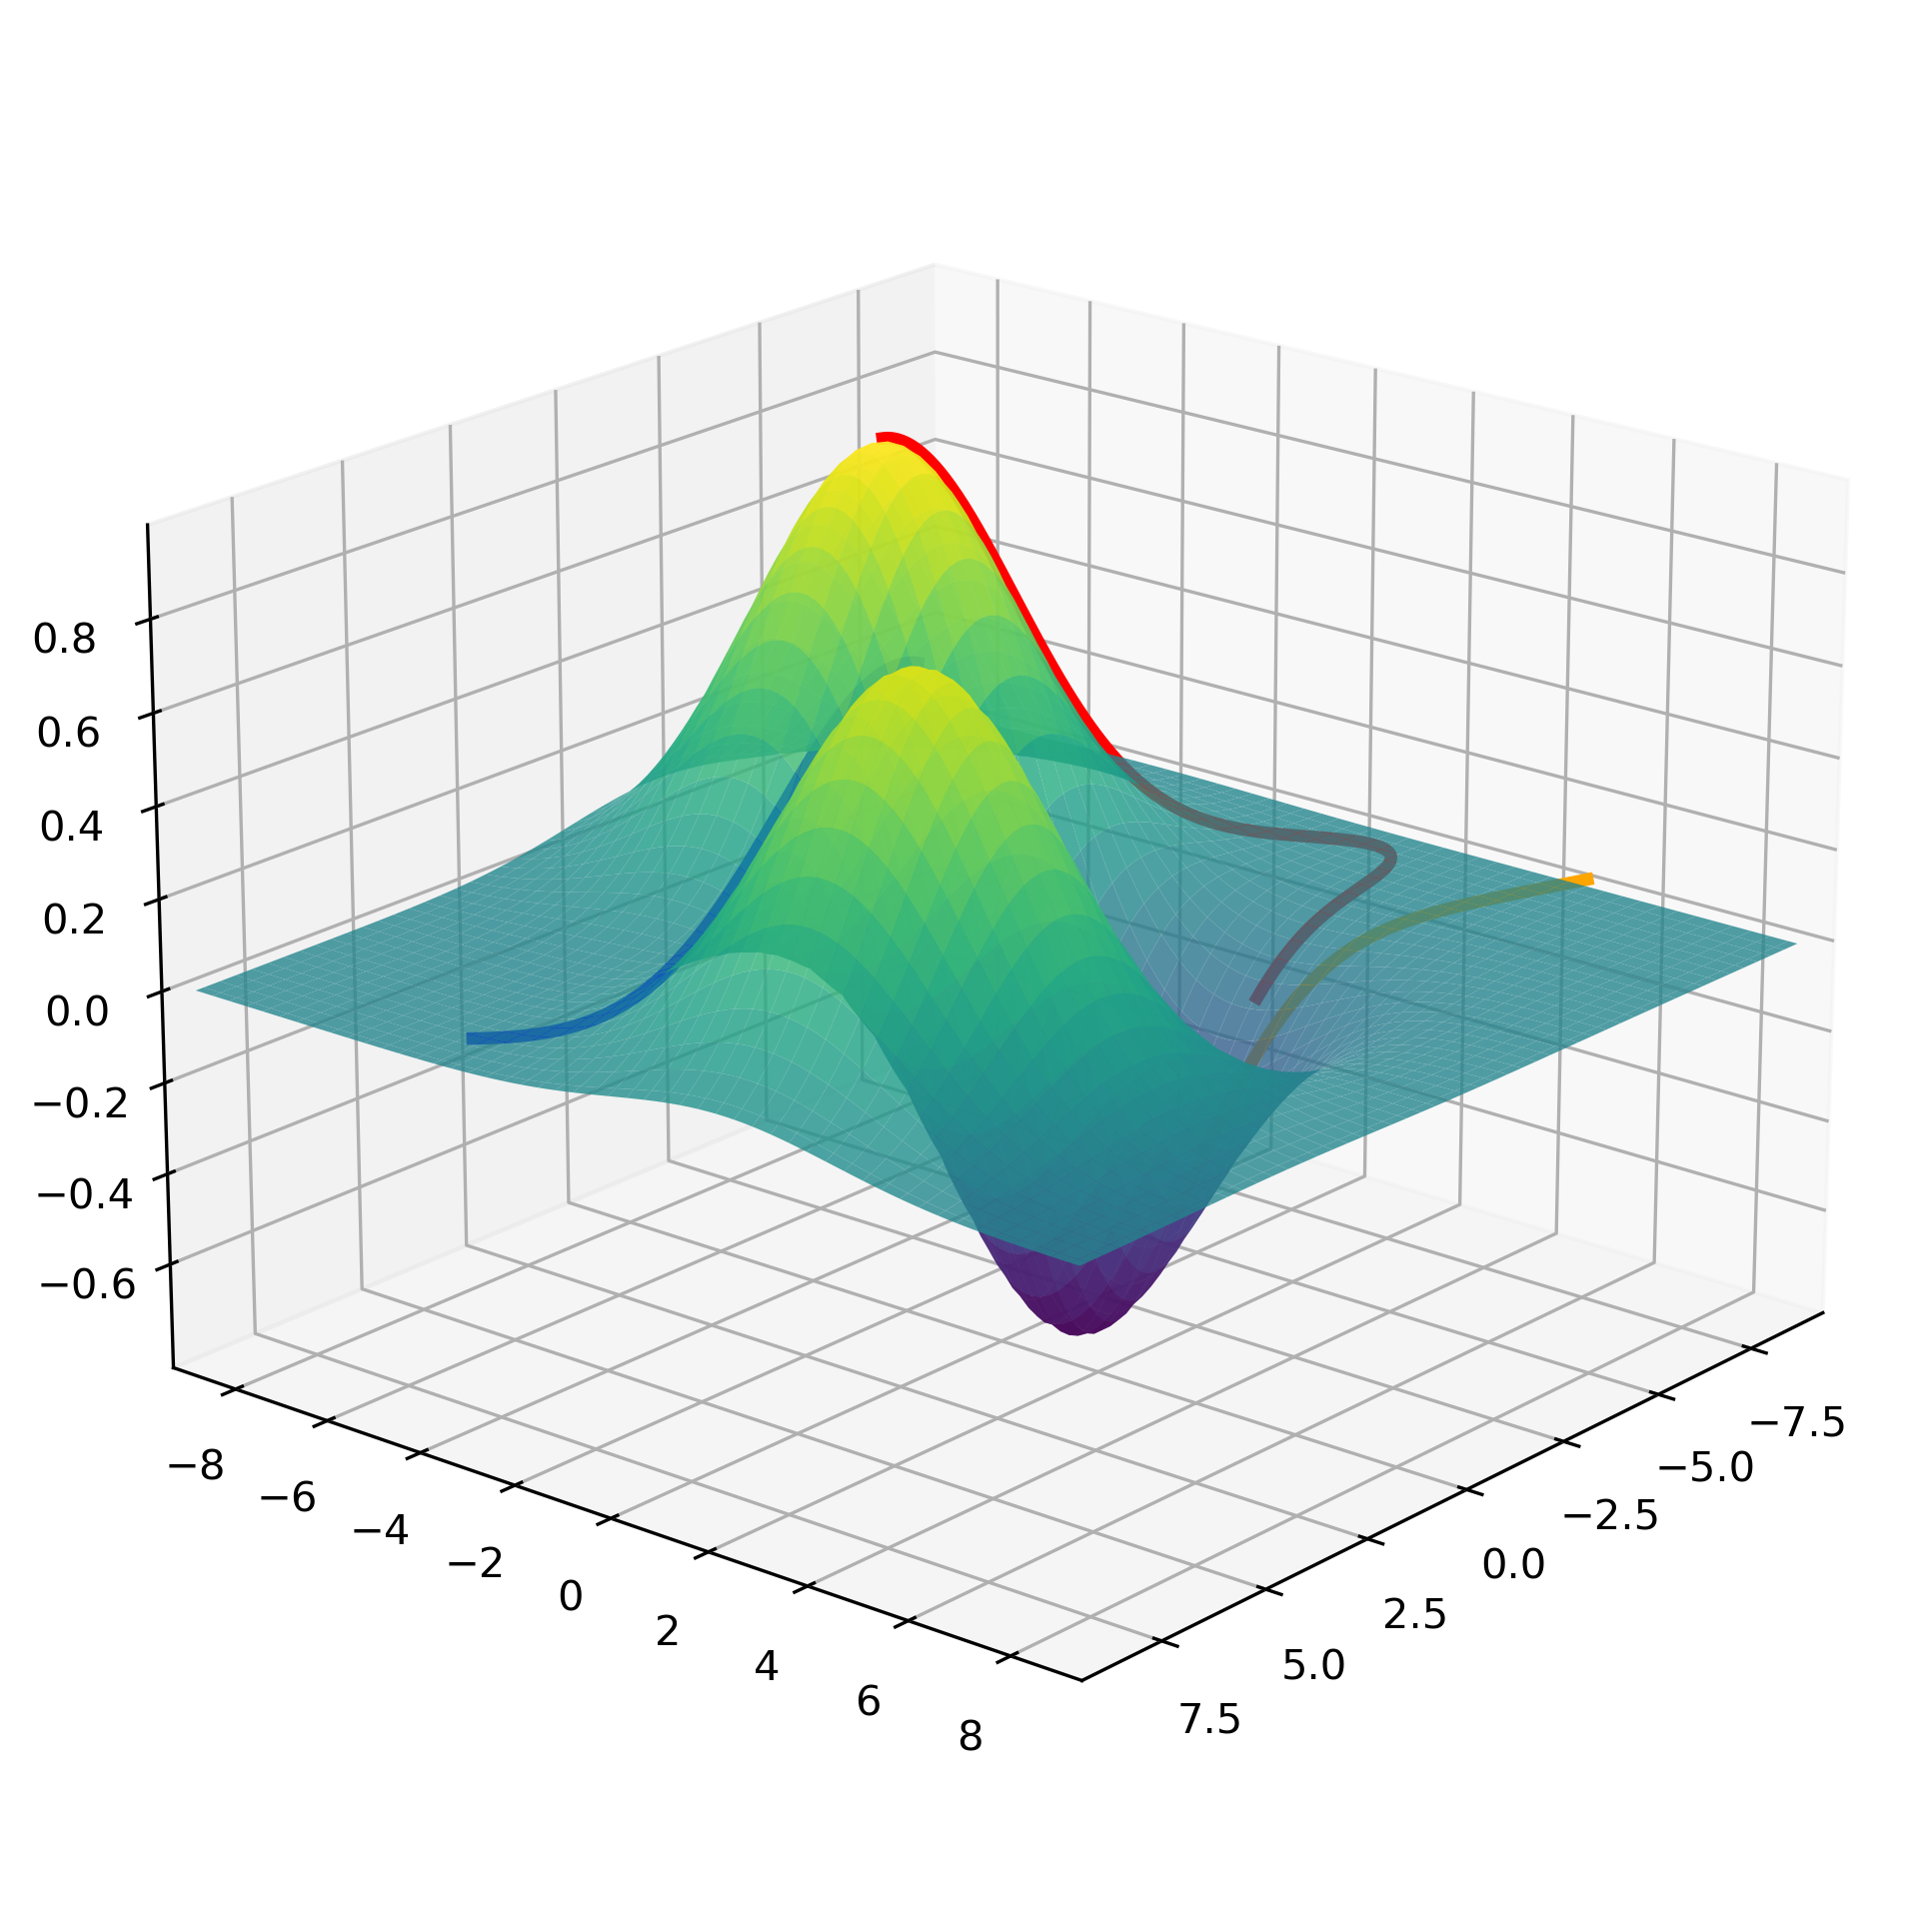
\includegraphics[scale=0.4]{notebooks/DL/img/3d_sgd.png}
    \caption{3D Plot}
\end{subfigure}%
\begin{subfigure}{.5\textwidth}
    \center
    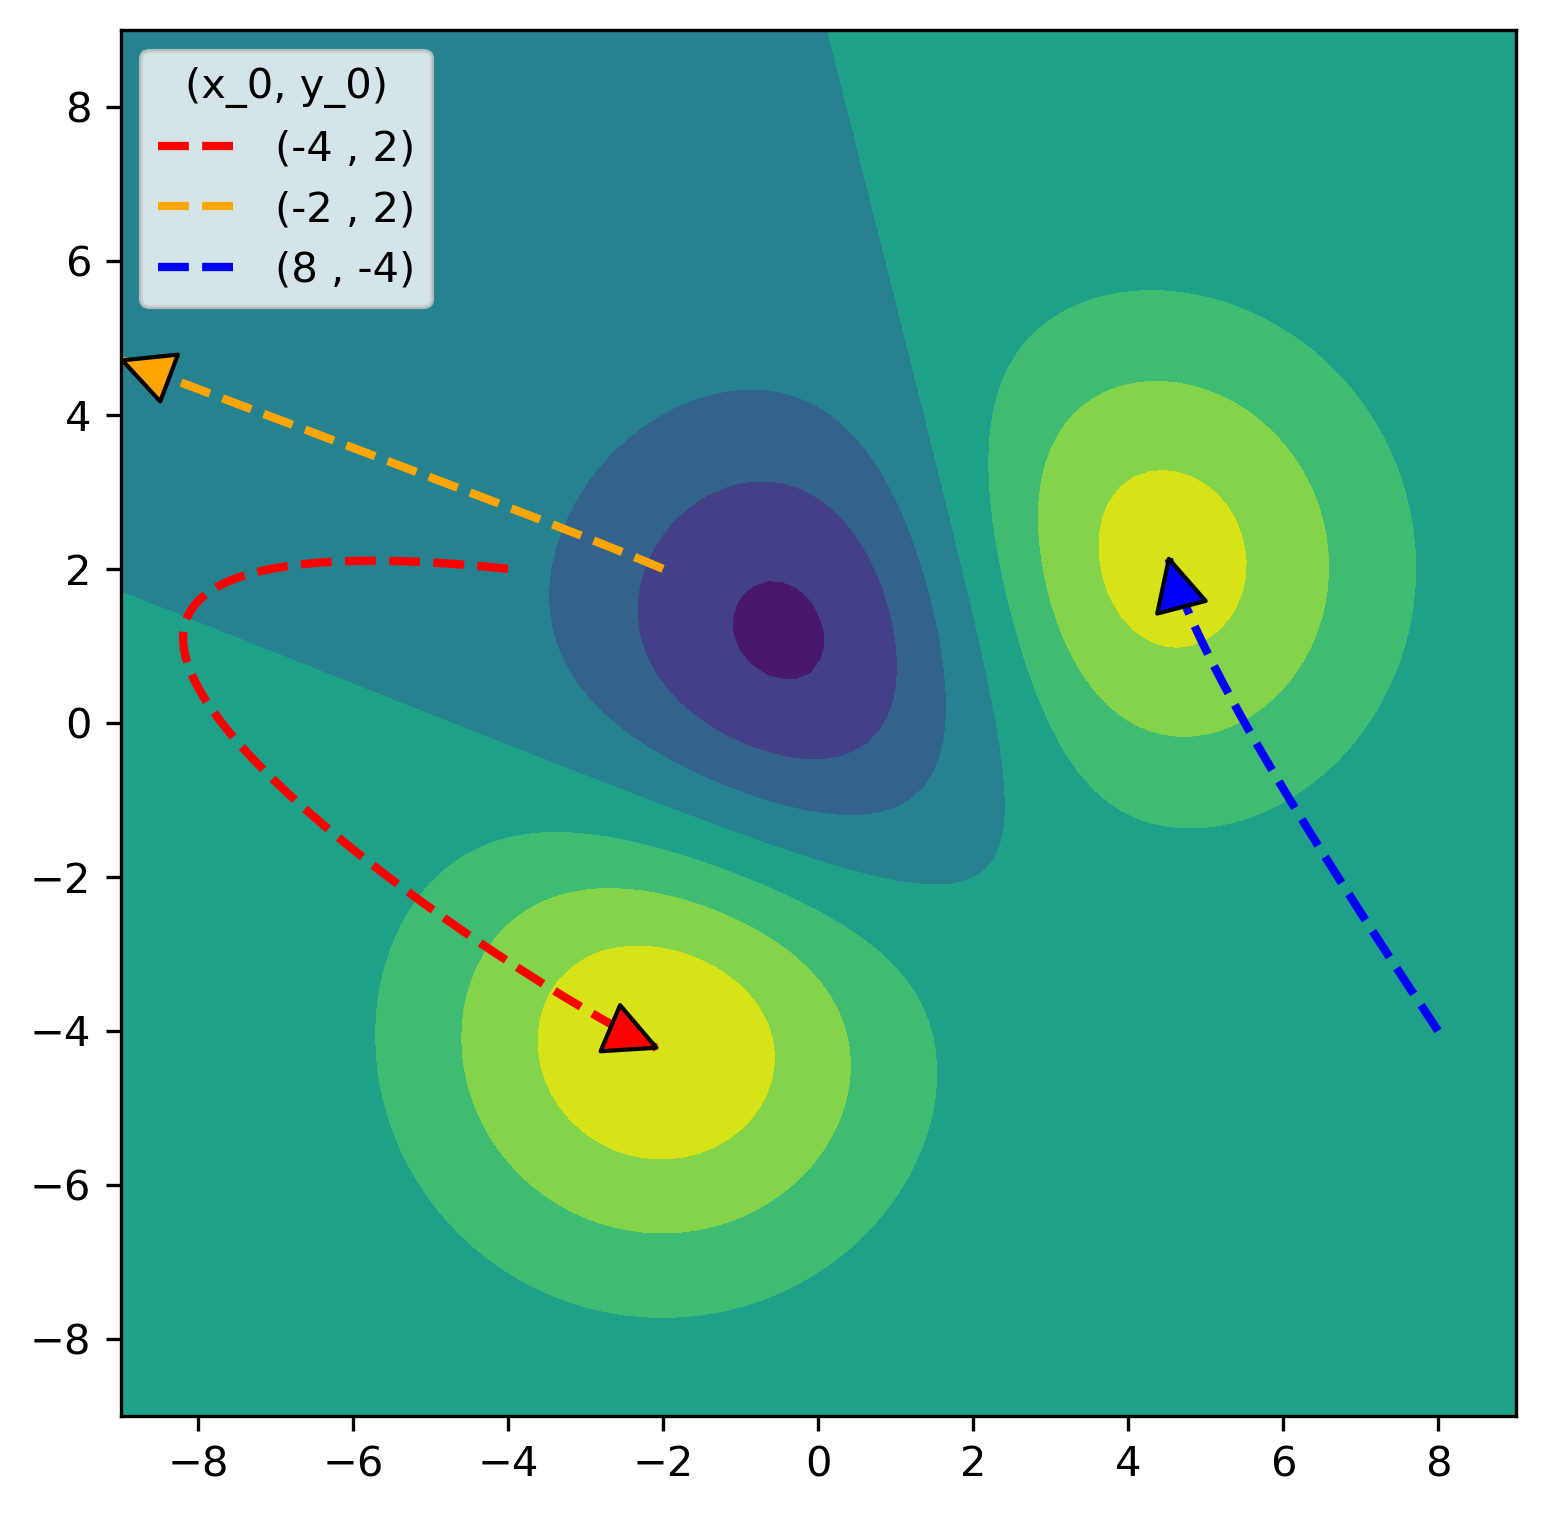
\includegraphics[scale=0.4]{notebooks/DL/img/contourf_sgd.png}
    \caption{Contour Plot}
\end{subfigure}
\caption{SGD Optimization for sum of Gaussian Distributions}
\end{figure}

\subsection{Stochastic Gradient Descent}

En problemas de Deep Learning, la función a minimizar $J$ dada una medida de desempeño $l(\hat{y},y) = l(f(x , \theta),y)$ se describe según 
$$ 
J^{*}(\theta) = \mathbb{E}_{(x,y) \sim p_{\text{data}}} l(f(x , \theta),y) .
$$
Que podemos aproximar por 
$$
J(\theta) = \mathbb{E}_{(x,y) \sim \hat{p}_{\text{data}}} l(f(x , \theta),y) = \frac{1}{k}\sum_{i=1}^{k}l(f(x_i , \theta),y_i)
$$
Con $k$ la cantidad de datos que consideremos en cada \textit{batch}. Entre menor sea el tamaño del batch, mayor será el ruido en la convergencia pero menor el costo computacional.

\begin{figure}[H]
    \center
    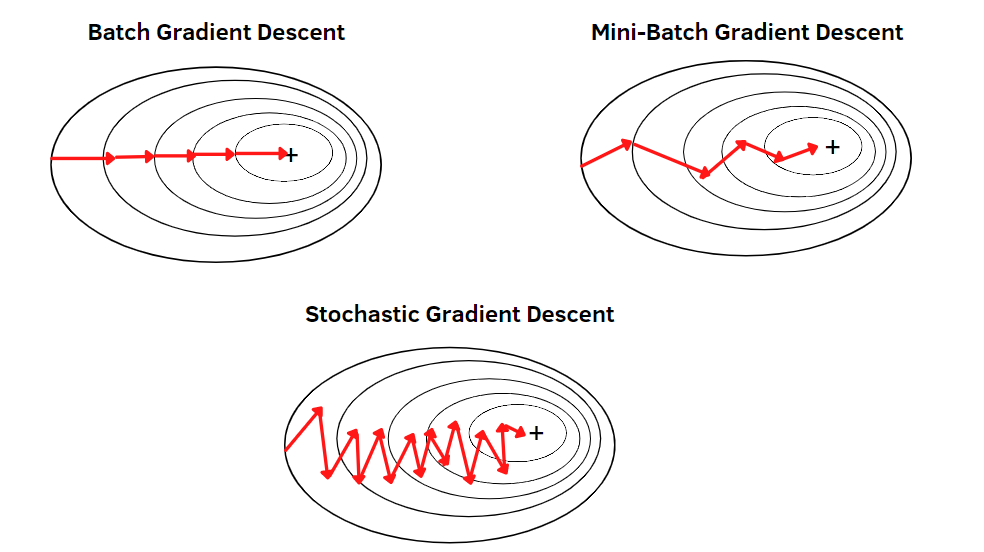
\includegraphics[scale=0.25]{notebooks/DL/img/sgd_diagram.png}
    \caption{SGD Diagram}
\end{figure}

